\documentclass[10pt]{article}

\usepackage[T1]{fontenc}
\usepackage[utf8]{inputenc}
\usepackage[english]{babel}
\usepackage{multicol}
\usepackage{amssymb,amsfonts,amsmath,amsthm}
\usepackage{graphicx}
\usepackage{lmodern}
\usepackage{cases}
\usepackage{pdfpages}
\usepackage{pgfplots}
\usepgfplotslibrary{colormaps}
\usepackage[margin=60pt]{geometry}
\usepackage{abstract}

\pgfplotsset{every axis/.append style={line width=1pt}}
\renewcommand{\abstractnamefont}{\normalfont\Large\bfseries}
\renewcommand{\abstracttextfont}{\normalfont\normalsize}

\usepackage{float}
\floatstyle{boxed}
\newfloat{boxframe}{H}{}
\floatname{boxframe}{Box}

\newcommand{\ud}{{\mathrm{d}}}
\newcommand{\pr}{{\mathbb{P}}}
\newcommand{\nN}{{n_\textrm{H}}}
\newcommand{\nI}{{n_\textrm{I}}}
\newcommand{\Xnema}{\textit{X. nematophila} }
\newcommand{\Scarpo}{\textit{S. carpocapsae} }
\newcommand{\Xenonema}{\textit{Xenorhabdus nematophila} }
\newcommand{\Steincarpo}{\textit{Steinernema carpocapsae} }
\newcommand{\Xeno}{\textit{Xenorhabdus} }
\newcommand{\Stein}{\textit{Steinernema} }
\newcommand{\Photo}{\textit{Photorhabdus} }
\newcommand{\Hetero}{\textit{Heterorhabditis} }
\newcommand{\IBD}{IBD}
\newcommand{\qw}{Q_\mathrm{w}}
\newcommand{\qb}{Q_\mathrm{b}}
\newcommand{\psis}{\psi_\mathrm{s}}
\newcommand{\psic}{\psi_\mathrm{c}}

\author{Latrille Thibault\\
\small thibault.latrille@ens-lyon.fr\\[-0.8ex]}
\title{Phenotypic variation as a cooperative strategy in \Xeno and \Photo} 
\begin{document}
%\includepdf[pages={1}]{first_page.pdf}
\begin{abstract}
Bacteria of the genus \Xeno and \Photo both colonize and influence the behavior of a nematode, \Stein and \Hetero respectively. The nematode infect, colonize and ultimately kills off an insect host, with the help of the bacteria. Thus the bacteria are symbiotic of two hosts, helping one to reproduce optimally while killing the other. Many studies focused on the symbiotic association between the bacteria and their respective and hosts, but they scarcely focused on cooperation at the bacterial level. We here provide evidence that the parasitic life cycle of these bacteria has a lot of influence on their relatedness, and thus on cooperation between bacteria. 
Cooperative evolutionary strategies of bacteria are investigated in the light of their symbiotic life cycle. We here provide ground on the occurrence that phenotypic variation, observed experimentally in both bacteria, is a cooperative strategy. We provide a very simple equation connecting phenotypic variation to relatedness. The relatedness is subsequently derived as a function of demographic parameters, experimentally accessible.
\smallskip
\noindent \textbf{Keywords.} symbioses, cooperation, \Xeno 
\end{abstract}
\begin{multicols}{2}
\section*{Introduction}
\begin{figure*}[hbt!]
	  \centering
	  \label{fig:life_cycle}
       \includegraphics[width=14.0cm]{Figures/life_cycle.png}\\
		\caption{ \textbf{The bacteria life cycle.} The infective juvenile nematode \Stein (\textit{Heterorhabditis}) containing \Xeno (\textit{Heterorhabditis}) bacteria (nematode–bacteria complex) enters a susceptible insect host through natural openings that include the mouth, anus and spiracles. After entering the insect blood system, the nematode releases the bacteria and develops into a fourth stage juvenile. The bacteria undergo an exponential growth until the population reaches approximately $10^9$ bacteria, the growth is followed by a plateau. Together, the nematode and bacteria overcome insect immunity and kill the insect. The insect cadaver is used as a nutrient source and is protected from opportunistic infection and scavenging by metabolites produced by bacteria. Within this environment, nematodes reproduce sexually and progeny develop through four juvenile stages. Some nematodes develop into infective juveniles after being recolonized by their respective bacteria. The pair then exit the depleted insect carcass in search of a new host.}
\end{figure*}
The $\gamma$-proteobacterium \Xenonema colonizes the entomopathogenic nematode \Steincarpo in a mutualistic association, and is also a pathogen of insects. 
The mutualistic relationship between \Xnema and \Scarpo is not obligate, as both partners can survive in the absence of the other; however, \Xnema is required for \Scarpo nematodes to reproduce efficiently during their lifecycle. 
\Scarpo nematodes are either found in insect hosts or in the soil. The soil-dwelling vector stage, called the infective juvenile (IJ), is encased in a double cuticle, and is non-feeding owing to its closed mouth and anus.
Prior to the IJ stage, ingested \Xnema bacteria colonize \Scarpo at a discrete intestinal location known as the vesicle. 
The IJ nematode then serves as a vector, carrying \Xnema into a susceptible insect, in which it is released from its nematode vector and rapidly kills the insect. 
\Xnema is capable of killing insects in the absence of \Scarpo by direct injection of \Xnema cells in the laboratory. 
\Xnema is capable of long-term survival in any reservoir outside its animal hosts in nature and, therefore, may rely on its nematode vector for transmission. 
The insect carcass provides nutrients for the propagation of both nematode and bacterium. 
In response to a signal, possibly nutrient deprivation or space limitation, \Xnema re-associates with the nematode, and the pair leave in search of a new insect host to repeat the cycle.
\Scarpo nematodes are easily propagated; several hundred thousand IJs can be generated from the infection of a single insect host or from lawns of X. nematophila and can be stored in water or buffer for weeks. 
Unlike many animals associated with bacterial mutualists, \Scarpo nematodes are viable in the absence of \Xnema Therefore, aposymbiotic nematodes can be obtained and assessed for responses to diverse bacterial and environmental stimuli. 
Haemolymph supports vigorous growth of X. nematophila (0.41 doublings per hour in haemolymph) even during release from the nematode. By contrast, the maximum \Xnema growth rate observed in the nematode vesicle was 0.1 doublings per hour, indicating that this environment is comparatively nutrient limiting.
The \Xnema population within an IJ nematode is founded by between one and two individual bacterial cells that grow to fill the vesicle, which is the lumen between two nematode epithelial cells at the anterior end of the intestine\cite{Martens}. The specificity is very stringent since other Xenorhabdus species do not colonize \Scarpo IJs.

Although \Xnema model is emerging as an invaluable tool for elucidating microorganism–host interactions. Many studies solely focused on the symbiotic association between the $\gamma$-protecterium and its hosts, but the scarcely discussed the cooperation at the bacterial level. We here provide evidence that the parasitic life cycle of these bacteria has a lot of influence on their relatedness. Thus evolutionary strategies of bacteria are investigated in the light of their symbiotic life cycle.

Relatedness is a key component of inclusive fitness, it is a measure of how closely two individuals are related. The relatedness is highly dependent on the genealogy of the population and of recent coalescent, thus population dynamic is closely related to relatedness. We here derived formulas for relatedness under several models of stochastic population dynamic. Deterministic approximation are made subsequently when calculus taking into account stochasticity become intractable. Our models seek to describe the biological case of a bacteria, the nematode-borne insect pathogen \Xnema.

The first section is dedicated to derive evolutionary strategies of bacteria as a function of relatedness. Subsequent section are devoted to derive the formula of the relatedness under two  model of infections of the insect by the nematodes. The former is considering all nematodes infect the insect simultaneously as propagules. The latter assume the nematodes arrive successively.

\section*{Fitness function and derivation of equilibrium.}
\begin{figure*}[hbt!]
	  \centering
	  \label{fig:fitness}
       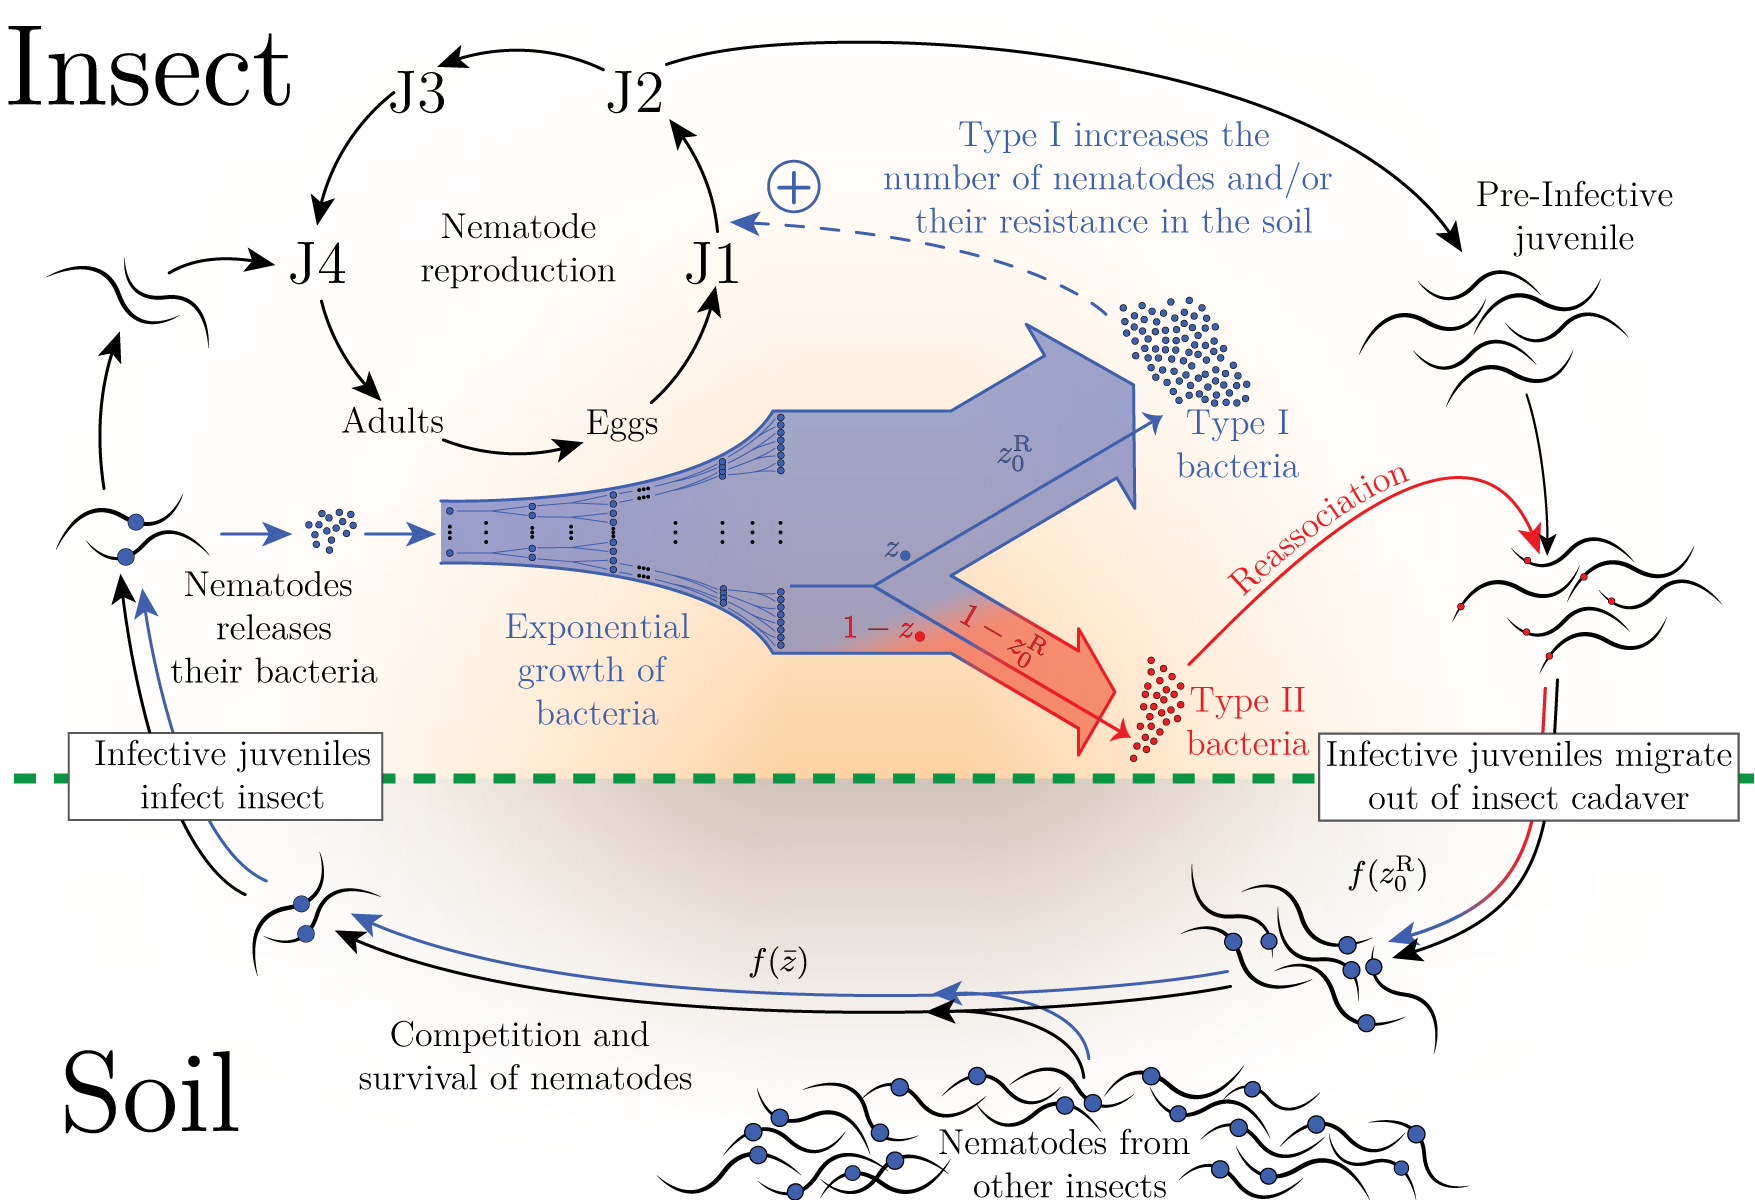
\includegraphics[width=14.0cm]{Figures/fitness.png}\\
		\caption{ \textbf{The bacteria cooperation along the life cycle.} The life cycle is the same as in figure \ref{fig:life_cycle} but we introduce phenotypic variation, namely type I and II. Type I are more virulent toward the insect, support nematode growth and development, kill off unwanted guests but cannot associate with the nematode. On the other hand, type II only associate to the nematode. The phenotype under investigation, $z_\bullet$ is the probability for one bacteria to switch from type I to type II. $z_0^{\mathrm{R}}$ is the proportion of type II in the insect, and the success of nematodes migrating out of the insect is $f(1- z_0^{\mathrm{R}})$. The average success of nematodes migrating out of all insects is $f(1- \bar{z})$. Thus the fitness of a focal bacterium is $z_\bullet f(1- z_0^{\mathrm{R}}) [f(1- \bar{z} ) z_0^{\mathrm{R}}]^{-1}$. We assume all bacteria switch back from type II to I during the soil dwelling stage.}
\end{figure*}

Indeed, both \Xeno and \Photo are found in the insect in two phenotypic variant \cite{Akhurst1982a,Forst1997}, denoted type I and II, controlled by a promoter inversion switch \cite{Somvanshi2012}. 
Type I are known to be more virulent toward the insect than type II \cite{Volgyi,Givaudan2000}. 
Type I are also known to produce crystal proteins \cite{Ciche2006,bintrim1998insertional} that supposedly nourish the nematode and support nematode growth and development \cite{Somvanshi2012}. 
And the nematode also feeds off the growing bacteria\cite{Waterfield2009}.  Type I also produces bactericides or fungicides that kill-off unwanted guests, thus increasing the foraging of the host by the nematodes.
On the other hand, type II bacteria are known to better associate with the nematode \cite{sicard2005effect}, by producing proteins involved in recognition by the nematode \cite{Somvanshi2010}. 
Moreover, studies have shown that nematodes did not emerge from insect when infected by type II solely \cite{Sugar2012}. 


We hereby intend to model this phenomenon, using simplifying assumptions in order to produce analytic prediction.  
In our model, type I are cooperators bacteria and type II are defectors\ref{fig:fitness}. 
We assume that type II die off in the insect but increase the number of nematodes that make it to the next cycle, or equivalently increase the survival of nematodes in the soil. 
However, a type I bacteria cannot colonize a nematode, and its fitness is null. 
On the other and type II are the one that can colonize the nematodes. 
The phenotype under investigation, $z$, is the probability of switching from type I to type II. We assume this phenotype is only expressed after the exponential growth of bacteria, which holds experimental grounds\cite{Somvanshi2012}.  We assume all bacteria switch back from type II to I during the soil dwelling stage of nematodes.
There is a trade off in this strategy. Indeed by switching to type II, a bacterium  increases its own fitness but decreases the fitness of related neighbors.  
A framework to study cooperative strategies is to consider inclusive fitness \cite{rousset2004genetic}.
To this aim, we identify three levels at which the phenotype has an impact on fitness:

$\bullet$ At the bacterial level, the phenotype is denoted $z_\bullet$.

$\bullet$ At the level of a population of bacteria inside the same insect. The average phenotype of the population is denoted $z_0^{\mathrm{R}}$. By definition, $z_0^{\mathrm{R}}$ is thus the proportion of type II in the insect, and $1-z_0^{\mathrm{R}}$ is the proportion of type I.

$\bullet$ At the level of the whole population of bacteria taking into account all the insects. The bacteria phenotype averaged over all insects is denoted $\bar{z}$. By definition, $1-\bar{z}$ is thus the proportion of type II over all insects, and $1-z_0^{\mathrm{R}}$ is the proportion of type I.

Thus for a focal bacterium, its success is $z_\bullet$ and the bacterium is competing with bacteria of average success $z_0^{\mathrm{R}}$. This bacterium is carried over by nematodes from the same insect, thus with success $f(1- z_0^{\mathrm{R}})$, competing with nematodes of average success $f(1- \bar{z} )$. We assume the success of nematodes $f$ is an increasing linear mapping of the proportion of type I: $f (z)=\alpha z+\beta$, $\alpha>0$.
  Putting together all the parts, and under the model of infinite number of insects, the fitness $w(z_\bullet ,z_0^{\mathrm{R}} , \bar{z} )$ of a focal bacterium is:
  \begin{align}
  w(z_\bullet ,z_0^{\mathrm{R}} , \bar{z} ) &= \dfrac{z_\bullet}{z_0^{\mathrm{R}}}\dfrac{f(1- z_0^{\mathrm{R}}) }{f(1- \bar{z} )} \\
  & = \dfrac{z_\bullet}{z_0^{\mathrm{R}}}\dfrac{\alpha+\beta-\alpha z_0^{\mathrm{R}}) }{\alpha+\beta-\alpha \bar{z}}
  \end{align}
  We then compute the partial derivative of the fitness with regard to $z_\bullet$ and $z_0^{\mathrm{R}}$ and evaluate them at $z$:
  \begin{equation}
   \left. \dfrac{\partial w(z_\bullet ,z_0^{\mathrm{R}} , \bar{z} )}{\partial z_\bullet} \right\vert_{z_\bullet = z_0^{\mathrm{R}} = \bar{z}=z} = \dfrac{1}{ z }.
  \end{equation}
  \begin{equation}
   \left. \dfrac{\partial w(z_\bullet ,z_0^{\mathrm{R}} , \bar{z} )}{\partial z_0^{\mathrm{R}}} \right\vert_{z_\bullet = z_0^{\mathrm{R}} = \bar{z}=z} = \dfrac{\alpha +\beta}{z(\alpha z -(\alpha+\beta))}.
  \end{equation}
  Let $R$ be the relatedness between bacteria. Following the framework of Rousset (2004) \cite{rousset2004genetic}, we yield a candidate evolutionary stable strategy depending on $R$:
    \begin{align}
    \left. \dfrac{\partial w}{\partial z_\bullet} \right\vert_{z^*} + \left. \dfrac{\partial w}{\partial z_0^{\mathrm{R}}} \right\vert_{z^*} R =0 \\
  \dfrac{1}{ z^* } + \dfrac{\alpha +\beta}{z(\alpha z^* -(\alpha+\beta))}R =0
  \end{align}
  \begin{equation}
  \iff
  \end{equation}
  \begin{equation}
  z^*=(1+\gamma)(1-R) \text{ where }\gamma=\dfrac{\beta}{\alpha}.
  \end{equation}
  In the special case $\gamma=0$ ($\beta=0$) the phenotype is equal to the complement of the relatedness:
  \begin{equation}
  z^*=1-R.
  \end{equation} 
  It is worth noting that if $R<\dfrac{\gamma}{\gamma+1}$, then the candidate evolutionary stable strategy is no cooperation $(z^*=1)$.
  The next section is dedicated to derive the relatedness $R$ under various models of migration and infection.
\section*{Relatedness as a function of demographic parameters.}
\subsection*{Simultaneous infections by propagules.}
Biologically, these assumption reflect the fact that we neglect competition, and also that the probability for a bacteria to divide is independent of its age.
The model is the following, $d$ nematodes infect an insect simultaneously (at time $t=0$). The probability of identity $\psis(t)$ is:
\begin{align}
\psis(t) &= \dfrac{ k_+ + \sum_{i=1}^d k_i^2}{k_+ (k_+ +1)}  -2 e^{-\lambda t} \dfrac{ k_+^2-\sum_{i=1}^d k_i^2}{k_+ (k_+^2 -1) }. 
\end{align}
Under the assumption $k_i \gg 1$, $ 1 \leq i \leq d $, the approximation of $\psis(t)$ becomes independent of $t$:
 \begin{equation}
\psis \simeq \displaystyle \sum_{i=1}^d \left( \dfrac{ k_i}{\sum_{i=1}^d k_i} \right)^2.
 \end{equation}
We also assume that each nematode carry the same number of bacteria. Mathematically, that is to say the $k_i$ are constant and equal $r$ for $0 \leq i \leq d$. The probability of identity $\psis$ reduces to:
\begin{equation}
\psis = \dfrac{1}{d}
\end{equation}
 This approximation is of particular interest. Indeed, providing the number of initial individual is large enough ($k_i \geq 100$), the probability of identity does not change over time and depends solely on the initial number of the nematodes. 
 \end{multicols}
\begin{boxframe}
\label{box_psi_simultaneous}
\begin{multicols}{2}
\textbf{Box 1. Proof of the equation \eqref{eqn:star}\\}
An insect is infected by $d$ nematodes. Each nematode $i$ ($ 1 \leq i \ d$) releases his bacteria inside the insect. The $d$ lineages of bacteria enter a stochastic growth process at time $t=0$.
In this context, $N_i(t)$ denote the discrete random variable describing the population size of the $i$th lineage at time $t$. $N_+(t)=\sum_{i=0}^d N_i(t)$ denote the discrete random variable describing the size of the whole population of bacteria at time $t$. The random variable $Z_i$ describe the event that two randomly chosen bacteria at time $t$ are from lineage $i$. By definition we have
\begin{equation}
Z_i=\dfrac{N_i(t)(N_i(t)-1)}{N_+(t)( N_+(t)-1 ) }.
\end{equation} 
The expectation of the sum of $Z_i$ over all lineages is thus $\psi (t)$, the expected odds 
at which two randomly chosen bacteria originate from the same nematode. 
\begin{equation}
\psi(t) = \mathbb{E} \left[ \sum_{i=1}^d Z_i(t) \right] = \sum_{i=1}^d \mathbb{E}[ Z_i(t)]
\end{equation}
Thus we need to evaluate $\mathbb{E}[ Z_i(t)]$. 
The growth process is modeled as a discrete space, continuous time Markov process. Each bacteria has an constant birth rate $\lambda$ and they never die, depicting an exponential growth. 
$k_i$ denote the number of bacteria initially contained by the $i$th nematode. The random variable $X_i(t)=N_i(t)-k_i$ is thus the number of births in the $i$th lineage. Under our model, 
$X_i(t)$ is a negative binomial\cite[p. 158]{cox1977theory}:
\begin{equation}
X_i(t) \sim \mathrm{NB} \left( k_i, e^{-\lambda t} \right) \iff
\end{equation}
\begin{equation}
\pr(X_i(t)=x)=\binom{x+k_i -1}{x} \left( e^{-\lambda t} \right)^{k_i} \left( 1-e^{-\lambda t} \right)^{x}.
\end{equation}
Consistently with previous denotation, $k_+=\sum_{i=0}^d k_i$ is the total number of bacteria released initially by the $d$ nematodes. Equivalently $X_+(t)=N_+(t)-k_+$ is the total number of bacteria born. Since all lineage of bacteria are independent of one another, $X_+(t)$ is also a negative binomial \cite{johnson2005univariate}:
\begin{equation}
 X_+(t)  \sim \mathrm{NB} \left( k_+, e^{-\lambda t} \right).
\end{equation}
Basic calculus leads to the distribution of $X_i(t)$ conditional on $ X_+(t)=x_+ $; this is a negative hypergeometric and independent of $e^{-\lambda t}$:
\begin{align}
\pr( X_i & (t) =x \vert X_+(t)=x_+ )  \nonumber \\ 
& = \dfrac{\displaystyle \binom{x+k_i-1}{x} \binom{x_+-x+k_+-k_i-1}{x_+-x}}{\displaystyle \binom{x_+ +k_+ -1}{x_+}}.
\end{align}
Leading to expectation for $X_i(t)(X_i(t)-1)$ conditional on $X_+(t)$:
\begin{align}
 \mathbb{E} [ X_i(t)& (X_i(t)-1) \vert X_+(t) ]  \nonumber \\
 &=\dfrac{k_i(k_i+1)}{k_+ (k_+ +1 )}X_+(t) ( X_+(t) -1 ).
\end{align}
And the expectation of $N_i(t)(N_i(t)-1)$ conditional on $N_+(t)$ is:
\begin{align}
 \mathbb{E} & [ N_i(t) (N_i(t)-1) \vert N_+(t) ]   \nonumber \\
 &=\dfrac{k_i(k_i+1) }{k_+ (k_+ +1)}N_+(t) ( N_+(t) -1 ) -\dfrac{2 k_i (k_+ - k_i) }{k_+ (k_+ +1)} N_+(t) .
\end{align}
Leading in turn to the expectation of $Z_i(t)$ conditional on $N_+(t)$.
\begin{align}
  \mathbb{E} [  Z_i(t)  & \vert N_+(t) ]  \nonumber \\
 &= \dfrac{k_i(k_i+1)}{k_+ (k_+ +1)}- \dfrac{2 k_i (k_+ -k_i)}{k_+ (k_+ +1)} \dfrac{1}{ N_+(t) -1  }.
\end{align}
By the law of conditional expectation:
\begin{align}
\mathbb{E}\left[ Z_i(t) \right] &= 
 \mathbb{E}\left[ \mathbb{E}\left[ \left. Z_i(t) \right\vert N_+(t) \right] \right]\\
 &=\dfrac{k_i(k_i+1)}{k_+ (k_+ +1 )}-\dfrac{2 k_i (k_+ -k_i)}{k_+ (k_+ +1 )}\mathbb{E}\left[\dfrac{1}{N_+(t)-1} \right] \\
 & =\dfrac{k_i(k_i+1)}{k_+ (k_+ +1 )}-2e^{-\lambda t}\dfrac{ k_i (k_+ -k_i)}{k_+ (k_+^2 -1 )}.
\end{align}
By summing $\mathbb{E}\left[ Z_i(t) \right]$ over all $i$, we evaluate the probability of identity $\psi(t)$:
\begin{equation}
\psi(t) =\dfrac{ k_+ + \sum_{i=1}^d k_i^2}{k_+ (k_+ +1)}  -2 e^{-\lambda t} \dfrac{ k_+^2-\sum_{i=1}^d k_i^2}{k_+ (k_+^2 -1) }.
\end{equation}
Under the assumption $k_i \gg 1$, $ 1 \leq i \leq d $, the approximation of $\psi(t)$ becomes independent of $t$:
 \begin{equation}
\psi \simeq \displaystyle \sum_{i=1}^d \left( \dfrac{ k_i}{\sum_{i=1}^d k_i} \right)^2.  \label{eqn:star} \tag{$\ast$}
 \end{equation}
 This approximation is of particular interest. Indeed, providing the number of bacteria carried by each nematode is large enough ($k_i \geq 100$), the probability of identity does not change over time and does not depend on 
 the bacteria growth rate.
 \end{multicols}
\end{boxframe}
\begin{multicols}{2}
The life cycle of the bacteria involve two hosts, nematodes and insects. The nematode is considered as the vector of the bacteria they carry around a hundred of them, and both are needed to infect the insect.
Let $Q_i$ be the probability of identity of genes from different bacteria, within the same insect ($\qw$) and in different insect ($\qb$). Here we consider the probability of identity 
in the infinite allele model, and let $u$ be the mutation rate.
 The recursion equations for next generation identities $\qw '$ and $\qb '$ are: 
  \begin{subnumcases}{\hspace*{-1.cm}}
      		 \qw ' = (1-u)^2[\psis + (1 -\psis) ( \phi \qw + (1-\phi) \qb ]  \\
    		 \qb ' = (1-u)^2 \left[ \dfrac{ \qw }{\nI}+\dfrac{\nI-1}{\nI} \qb \right].
  \end{subnumcases}
  At equilibrium, $\qw ' = qw$ and $\qb ' =\qb$ and the recursion equations are:
  \begin{subnumcases}{\hspace*{-1cm}}
      		 \qw = (1-u)^2[\psis + (1 -\psis) ( \phi \qw + (1-\phi) \qb ] \\
    		 \qb = (1-u)^2 \left[ \dfrac{ \qw }{\nI}+\dfrac{\nI-1}{\nI} \qb \right].
  \end{subnumcases}
  This simultaneous can be solved unambiguously and leads to the relatedness
  \begin{align}
 R &= \dfrac{\qw - \qb }{ 1- \qb } \\
 &= \dfrac{ \psis (1-u)^2 }{ 1 - (1-u)^2 \phi (1- \psis )+(1-u)^2 / \nI } .
 \end{align}
And thus by taking the limit for low mutation rate ($u \rightarrow 0$), the relatedness becomes:
 \begin{equation}
 R \simeq \dfrac{ \psis  }{ 1 - \phi (1- \psis )+1 / \nI }.
 \end{equation} 
Under the assumption of an important number of demes ($\nI \rightarrow \infty$), the relatedness $R$ is:
 \begin{equation}
 R \simeq \dfrac{ \psis  }{ 1 - \phi (1- \psis ) }
 \end{equation}
 \begin{figure}[H]
\label{fig:R}
\centering
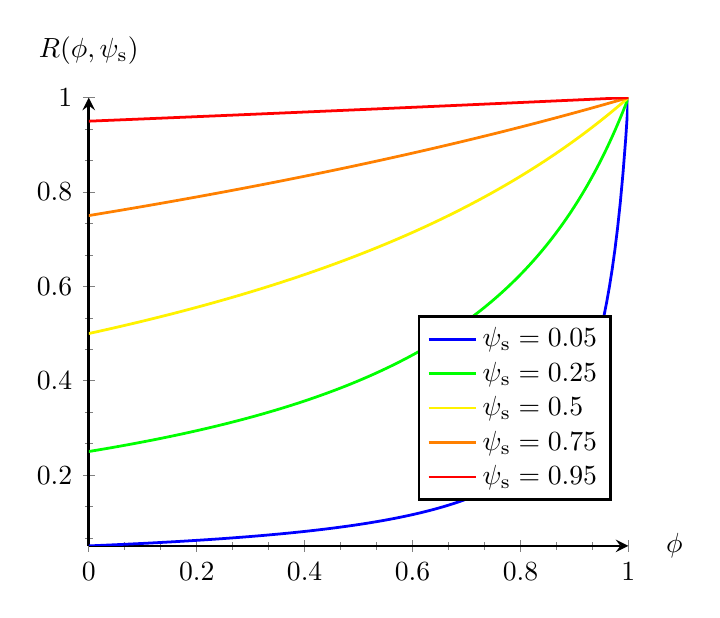
\begin{tikzpicture}
\begin{axis}[
ylabel={$R(\phi,\psis)$},
xlabel={$\phi$},
domain=0:1,
samples=201,
legend entries={$\psis=0.05$,$\psis=0.25$, $\psis=0.5$,$\psis=0.75 $,$\psis=0.95 $},
legend cell align=left,
minor tick num=2,
axis x line=bottom,
axis y line=left,
every axis x label/.style={
    at={(ticklabel* cs:1.05)},
    anchor=west,
},
every axis y label/.style={
    at={(ticklabel* cs:1.05)},
    anchor=south,
},
legend style={at={(0.97,0.1)},anchor=south east}
]
\addplot[blue]{0.05 /(1 - (1 - 0.05)* x)};
\addplot[green]{.25 /(1 - (1 - 0.25)* x)};
\addplot[yellow]{0.5 /(1 - (1 - 0.5)* x)};
\addplot[orange]{0.75 /(1 - (1 - 0.75)* x)};
\addplot[red]{0.95 /(1 - (1 - 0.95)* x)};
\end{axis}
\end{tikzpicture}
\caption{\textbf{Relatedness as a function of $\psis$ and $\psi$.} Plot of the relatedness against $\phi$ for several values of $\psis$ ranging from $0.05$ to $0.95$. $\psi$ is blabla and $\phi$ is blabla}
\end{figure}
\subsection*{Consecutive infections.}
  We derive the formula for two nematodes arriving at different times. We assume nematodes arrive at times exponentially distributed of parameter $ \tau$. If we assume the lineage carried by the first vector grew in a deterministic fashion, then its size is $r e^{\lambda  T}$. $\omega=\tau / \lambda$
\begin{equation}
   \psic (\omega)= 1- 2 \omega \mathrm{B}_{1/2}(1+\omega,1-\omega), \label{psic_consecutive}
\end{equation}
where $\mathrm{B}_x(a,b)$ is the incomplete beta function:
\begin{align}
\mathrm{B}_x(a,b) = \int_0^x t^{a-1}(1-t)^{b-1} \ud t.
\end{align}
Calculus become intractable when there is more than two nematodes arriving in the insect. Computation shows that the deterministic approximation is quite good and that for more than two nematodes, the shape is quite the same too.
\begin{figure}[H]
\label{fig:psic}
\centering
\begin{tikzpicture}
\begin{axis}[
xlabel={$\omega$},
ylabel={$\hat{\psic}$},
ymin=0.2, ymax=1,
legend cell align=left,
minor tick num=2,
axis x line=bottom,
axis y line=left,
every axis x label/.style={
    at={(ticklabel* cs:1.05)},
    anchor=west,
},
every axis y label/.style={
    at={(ticklabel* cs:1.05)},
    anchor=south,
},
legend style={at={(1,0.95)},anchor=north east}
] \addplot[black, no markers] coordinates {(0,0.5) (5,0.5)};
\addplot[black, no markers] coordinates {(0,0.333) (5,0.333)};
\addplot[black, no markers] coordinates {(0,0.25) (5,0.25)};
\addplot[blue] table[x index=0,y index=2,col sep=space] {3nematodes_randtime_randgrowth.txt};
\addlegendentry{Mean for 3 nematodes}
\addplot[purple] table[x index=0,y index=2,col sep=space] {4nematodes_randtime_randgrowth.txt};
\addlegendentry{Mean for 4 nematodes}
\addplot[green] table[x index=0,y index=3,col sep=space] {2nematodes_randtime_randgrowth.txt};
\addlegendentry{Lower interval}
\addplot[red] table[x index=0,y index=4,col sep=space] {2nematodes_randtime_randgrowth.txt};
\addlegendentry{Upper interval}
\addplot[black] table[x index=0,y index=1,col sep=space] {coucou.dat};
\addlegendentry{$1- 2 \omega \mathrm{B}_{1/2}(1+\omega,1-\omega)$}
\end{axis}
\end{tikzpicture}
\caption{\textbf{The analytic formula of $\psic$ compared to simulated results}$\psic$ is depicted in figure \ref{fig:psic} as long as simulated data taking into account stochastic growth of bacteria.}
\end{figure}
\end{multicols}
\begin{boxframe}
\label{box_psi_consecutive}
\begin{multicols}{2}
\textbf{Box 2. Proof of  the formula \eqref{eqn:star2}\\}
We derive an analytic formula of $\psic$ for two nematodes arriving successively. We assume nematodes arrive at times exponentially distributed of parameter $ \tau$. Thus, the first nematode arrive at time $T$ before the second (and last) nematode, where $T\sim \exp ( \tau)$. We also assume assume each nematode carries the same number of bacteria, $k \gg 1$. And finally, we assume the bacteria carried by the nematodes grew in a deterministic fashion at rate $\lambda$. Under all these assumptions, the number of bacteria in the insect when the second nematode arrives is the random variable $k e^{\lambda  T}+k$. Where $k e^{\lambda  T}$ bacteria are from the first one arrived and $k$ are from the second one.\\ 
  Since $k \gg 1$, the random variable $k e^{\lambda  T} $ is always far greater than $1$. Thus we can make use of the equation \eqref{eqn:star} to derive $\psic$:
  \begin{align}
  \psic  &=\mathbb{E} \left[ \left( \dfrac{ k e^{\lambda T}}{k+ke^{\lambda T}} \right)^2+\left( \dfrac{k}{k+ke^{\lambda T}} \right)^2 \right] \\
  &=\mathbb{E} \left[ \left( \dfrac{ e^{\lambda T}}{1+e^{\lambda T}} \right)^2+\left( \dfrac{1}{1+e^{\lambda T}} \right)^2 \right] \\
  &=\int_0^\infty \left( \left( \dfrac{ e^{\lambda t}}{1+e^{\lambda t}} \right)^2 + \left( \dfrac{1}{1+e^{\lambda t}} \right)^2 \right) \tau e^{ -\tau t } \ud t.
  \end{align}
  The evaluation of this integral is not straightforward. Instead we derive the cumulative distribution function $F_1(p)$ and $F_2(p)$, and the probability density function $f_1(p)$ and $f_2(p)$ of $\dfrac{ e^{\lambda T}}{1+e^{\lambda T}}$ and $\dfrac{ 1}{1+e^{\lambda T}}$ respectively.
  \begin{align}
  F_1(p) &= \pr \left(\dfrac{e^{\lambda T}}{1+e^{\lambda T}} \leq p\right)= \pr \left(T \leq \lambda^{-1} \mathrm{ln}\left( \dfrac{p}{1-p} \right) \right) \nonumber \\
  &= 1-(1-p)^{\omega} p^{-\omega} \text{ for } 1/2 \leq p \leq 1,
  \end{align} 
  where $\omega=\tau / \lambda$.
  \begin{align}
  F_2(p) &= \pr \left(\dfrac{1}{1+e^{\lambda T}} \leq p\right) = \pr \left(T \geq \lambda^{-1} \mathrm{ln}\left( \dfrac{1-p}{p} \right) \right) \nonumber \\
  &= (1-p)^{-\omega} p^\omega \text{ for } 0 \leq p \leq 1/2.
  \end{align}
  And the probability density function $f_1(p)$ and $f_2(p)$ are:
  \begin{align}
  f_1(p) &= \dfrac{ \ud F_1(p) }{ \ud p} =  \omega (1-p)^{\omega-1} p^{-\omega-1}  \text{ for } 1/2 \leq p \leq 1\\
  f_2(p) &= \dfrac{ \ud F_2(p) }{ \ud p} =  \omega (1-p)^{-\omega-1} p^{\omega-1} \text{ for } 0 \leq p \leq 1/2.
  \end{align}
  And 
  \begin{align}
  \psic (\omega)&= \int_{1/2}^{1} p^2 f_1(p) \ud p + \int_{0}^{1/2} p^2 f_2(p) \ud p \\
  &= 1 -2  \omega \int_{0}^{1/2}  (1-x)^{-\omega} x^{\omega}  \ud x \\
  &= 1- 2 \omega \mathrm{B}_{1/2}(1+\omega,1-\omega). \label{eqn:star2} \tag{ $\ast \ast$ }
  \end{align}
  where $\mathrm{B}_x(a,b)$ is the incomplete beta function:
\begin{align}
\mathrm{B}_x(a,b) = \int_0^x t^{a-1}(1-t)^{b-1} \ud t.
\end{align}
  Thus the probability of identity is solely dependent on one parameter, $\omega$, the ratio between arrival rate of nematodes and growth rate of bacteria. 
  $\psic (\omega)$ is depicted in figure \ref{fig:psic} as long as simulated data taking into account stochastic growth of bacteria.
 \end{multicols}
\end{boxframe}
\begin{multicols}{2}
Taking mutation rate $u$ into account, in a similar fashion to \cite{rousset2004genetic}, the recursion equations are: 
  \begin{subnumcases}{\hspace*{-1cm}}
      		\qw ' = (1-u)^2 \left[ \psic + \left( \dfrac{ \qw }{\nI}+\dfrac{\nI-1}{\nI} \qb \right) (1 -\psic) \right] \\
    		\qb ' = (1-u)^2 \left[ \dfrac{ \qw }{\nI}+\dfrac{\nI-1}{\nI} \qb \right].
  \end{subnumcases}
 At equilibrium, $\qw ' = \qw$ and $\qb ' =\qb$ and the recursion equations are:
  \begin{subnumcases}{\hspace*{-1cm}}
      		\qw = (1-u)^2 \left[ \psic + \left( \dfrac{\qw}{\nI}+\dfrac{\nI-1}{\nI} \qb \right) (1 -\psic) \right] \\
    		\qb = (1-u)^2 \left[ \dfrac{\qw}{\nI}+\dfrac{\nI-1}{\nI} \qb \right].
  \end{subnumcases}
 Leading to the unique solution:
   \begin{subnumcases}{\hspace*{-1cm}}
 \qw = \dfrac{ (1-u)^2 [u (2 - u)(\nI-1) +1 ]\psic }{ u (2-u )(\nI - \psic )+\psic }\\
 \qb = \dfrac{(1- u )^4 \psic}{u (2-u) (\nI - \psic ) +\psic}.
  \end{subnumcases}
 And the relatedness is: 
 \begin{align}
 R &= \dfrac{\qw - \qb }{1- \qb} \\
   &=\dfrac{(1-u)^2 \nI \psic}{\nI +(1-u)^2 \psic}.
 \end{align}
And thus by taking the limit for low mutation rate ($u \rightarrow 0$), the relatedness becomes:
 \begin{equation}
 R \simeq \dfrac{\psic}{1+ \dfrac{\psic}{\nI}}.
 \end{equation} 
Under the assumption of an important number of demes ($\nI \rightarrow \infty$), the relatedness is:
 \begin{equation}
 R \simeq \psic 
 \end{equation}
 It is worth noting that the relatedness does not depend on the number of bacteria initially brought by the nematode ($r$), nor on the the total population size when the bacteria stop growing exponentially. 
 This formula is valid only if the population of bacteria is growing exponentially at the time the last nematode infected the insect.
\section*{Discussion}
There is no experimental barrier to manipulate parameters such as $\phi$ or the number of nematodes infecting the insects in the lab. Thus if our theoretical model describe with enough accuracy the underlying biological model, \Xnema is invaluable model for studying cooperation for numerous reasons. 
Only one bacteria enters the nematode thus they are all clones once liberated in the insect. 
\section*{Acknowledgments}
\bibliographystyle{plain}
\bibliography{References_none_mendeley,References}
\end{multicols}
\end{document}

% \begin{tikzpicture}
%\begin{axis}[
%view={-45}{45},
%colorbar horizontal,
%colormap/temp,
%title={$R \simeq \dfrac{ \psi  }{ 1 - \phi (1- \psi )}$},
%xlabel={$\psi$},
%ylabel={$\phi$},
%]
%\addplot3[
%surf,
%domain=0:1,
%domain y=0:1,
%shader=faceted interp,
%draw=black,
%]
%{x /(1 - (1 - x)* y)};
%\end{axis}
%\end{tikzpicture}